\documentclass[tikz,border=8pt]{standalone}
\usepackage[utf8]{inputenc}
\usepackage[T1]{fontenc}
\usepackage{lmodern}
\usetikzlibrary{arrows.meta,positioning,fit}
\definecolor{navy}{HTML}{15324B}
\definecolor{blue}{HTML}{2F80C1}
\definecolor{cyan}{HTML}{DCEFF7}
\definecolor{orange}{HTML}{E8873A}
\definecolor{green}{HTML}{3B8F72}
\tikzset{
 box/.style={draw=navy,rounded corners=3pt,very thick,minimum width=3.1cm,minimum height=1.25cm,align=center,fill=white,font=\sffamily},
 arrow/.style={-{Latex[length=3mm]},very thick,draw=navy},
 note/.style={font=\sffamily\small,align=center,text=navy}
}
\begin{document}
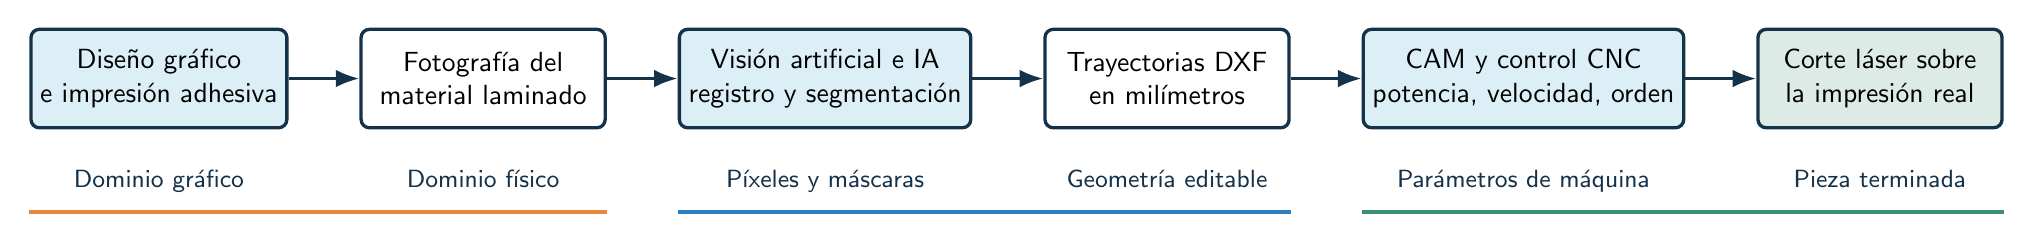
\begin{tikzpicture}[node distance=1.0cm and 0.9cm]
\node[box,fill=cyan] (design) {Diseño gráfico\\e impresión adhesiva};
\node[box,right=of design] (capture) {Fotografía del\\material laminado};
\node[box,right=of capture,fill=cyan] (vision) {Visión artificial e IA\\registro y segmentación};
\node[box,right=of vision] (vector) {Trayectorias DXF\\en milímetros};
\node[box,right=of vector,fill=cyan] (cam) {CAM y control CNC\\potencia, velocidad, orden};
\node[box,right=of cam,fill=green!18] (cut) {Corte láser sobre\\la impresión real};
\draw[arrow] (design)--(capture);
\draw[arrow] (capture)--(vision);
\draw[arrow] (vision)--(vector);
\draw[arrow] (vector)--(cam);
\draw[arrow] (cam)--(cut);
\node[note,below=0.4cm of design] {Dominio gráfico};
\node[note,below=0.4cm of capture] {Dominio físico};
\node[note,below=0.4cm of vision] {Píxeles y máscaras};
\node[note,below=0.4cm of vector] {Geometría editable};
\node[note,below=0.4cm of cam] {Parámetros de máquina};
\node[note,below=0.4cm of cut] {Pieza terminada};
\draw[orange,very thick] ([yshift=-1.05cm]design.south west)--([yshift=-1.05cm]capture.south east);
\draw[blue,very thick] ([yshift=-1.05cm]vision.south west)--([yshift=-1.05cm]vector.south east);
\draw[green,very thick] ([yshift=-1.05cm]cam.south west)--([yshift=-1.05cm]cut.south east);
\end{tikzpicture}
\end{document}
